\tikzset{every picture/.style={line width=0.75pt}} %set default line width to 0.75pt        

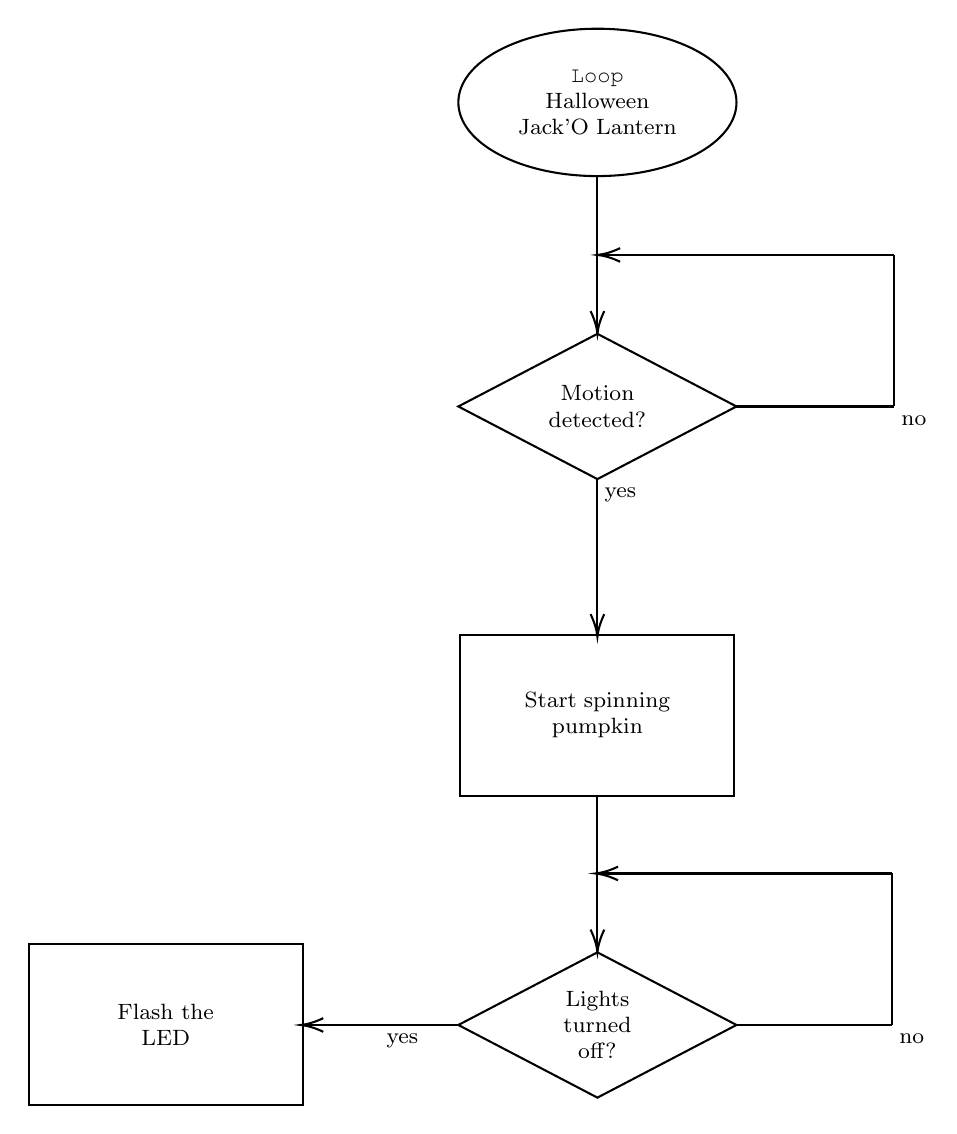
\begin{tikzpicture}[x=0.75pt,y=0.75pt,yscale=-1,xscale=1]
%uncomment if require: \path (0,613); %set diagram left start at 0, and has height of 613

%Shape: Ellipse [id:dp4933232876887643] 
\draw   (264,37.5) .. controls (264,17.89) and (294,2) .. (331,2) .. controls (368,2) and (398,17.89) .. (398,37.5) .. controls (398,57.11) and (368,73) .. (331,73) .. controls (294,73) and (264,57.11) .. (264,37.5) -- cycle ;
%Straight Lines [id:da26842845788901504] 
\draw    (331,73) -- (331,147) ;
\draw [shift={(331,149)}, rotate = 270] [color={rgb, 255:red, 0; green, 0; blue, 0 }  ][line width=0.75]    (10.93,-3.29) .. controls (6.95,-1.4) and (3.31,-0.3) .. (0,0) .. controls (3.31,0.3) and (6.95,1.4) .. (10.93,3.29)   ;
%Shape: Diamond [id:dp5887414211572617] 
\draw   (331,149) -- (398,184) -- (331,219) -- (264,184) -- cycle ;
%Straight Lines [id:da11949718861713432] 
\draw    (474,111) -- (333,111) ;
\draw [shift={(331,111)}, rotate = 360] [color={rgb, 255:red, 0; green, 0; blue, 0 }  ][line width=0.75]    (10.93,-3.29) .. controls (6.95,-1.4) and (3.31,-0.3) .. (0,0) .. controls (3.31,0.3) and (6.95,1.4) .. (10.93,3.29)   ;
%Shape: Boxed Line [id:dp8672990347188025] 
\draw    (474,184) -- (398,184) ;
%Straight Lines [id:da3501871976442579] 
\draw    (474,111) -- (474,184) ;
%Straight Lines [id:da6443564757215938] 
\draw    (331,219) -- (331,293) ;
\draw [shift={(331,295)}, rotate = 270] [color={rgb, 255:red, 0; green, 0; blue, 0 }  ][line width=0.75]    (10.93,-3.29) .. controls (6.95,-1.4) and (3.31,-0.3) .. (0,0) .. controls (3.31,0.3) and (6.95,1.4) .. (10.93,3.29)   ;
%Shape: Rectangle [id:dp3254676452627636] 
\draw   (265,294) -- (397,294) -- (397,371.5) -- (265,371.5) -- cycle ;
%Straight Lines [id:da8857219457937153] 
\draw    (331,371) -- (331,445) ;
\draw [shift={(331,447)}, rotate = 270] [color={rgb, 255:red, 0; green, 0; blue, 0 }  ][line width=0.75]    (10.93,-3.29) .. controls (6.95,-1.4) and (3.31,-0.3) .. (0,0) .. controls (3.31,0.3) and (6.95,1.4) .. (10.93,3.29)   ;
%Shape: Diamond [id:dp36813807481182326] 
\draw   (331,447) -- (398,482) -- (331,517) -- (264,482) -- cycle ;
%Straight Lines [id:da38280033743458897] 
\draw    (473,409) -- (332,409) ;
\draw [shift={(330,409)}, rotate = 360] [color={rgb, 255:red, 0; green, 0; blue, 0 }  ][line width=0.75]    (10.93,-3.29) .. controls (6.95,-1.4) and (3.31,-0.3) .. (0,0) .. controls (3.31,0.3) and (6.95,1.4) .. (10.93,3.29)   ;
%Shape: Boxed Line [id:dp34281321927853337] 
\draw    (473,482) -- (397,482) ;
%Straight Lines [id:da2693019447857199] 
\draw    (473,409) -- (473,482) ;
%Straight Lines [id:da26427822519290967] 
\draw    (264,482) -- (190,482) ;
\draw [shift={(188,482)}, rotate = 360] [color={rgb, 255:red, 0; green, 0; blue, 0 }  ][line width=0.75]    (10.93,-3.29) .. controls (6.95,-1.4) and (3.31,-0.3) .. (0,0) .. controls (3.31,0.3) and (6.95,1.4) .. (10.93,3.29)   ;
%Shape: Rectangle [id:dp7355929762130229] 
\draw   (57,443) -- (189,443) -- (189,520.5) -- (57,520.5) -- cycle ;

% Text Node
\draw (331,37.5) node  [font=\footnotesize] [align=left] {\begin{minipage}[lt]{57.35pt}\setlength\topsep{0pt}
\begin{center}
{\fontfamily{pcr}\selectfont Loop}\\Halloween\\Jack'O Lantern
\end{center}

\end{minipage}};
% Text Node
\draw (331,184) node  [font=\footnotesize] [align=left] {\begin{minipage}[lt]{38.57pt}\setlength\topsep{0pt}
\begin{center}
Motion \\detected?
\end{center}

\end{minipage}};
% Text Node
\draw (476,187) node [anchor=north west][inner sep=0.75pt]  [font=\footnotesize] [align=left] {no};
% Text Node
\draw (333,222) node [anchor=north west][inner sep=0.75pt]  [font=\footnotesize] [align=left] {yes};
% Text Node
\draw (331,332.75) node  [font=\footnotesize] [align=left] {\begin{minipage}[lt]{52.63pt}\setlength\topsep{0pt}
\begin{center}
Start spinning\\pumpkin
\end{center}

\end{minipage}};
% Text Node
\draw (331,482) node  [font=\footnotesize] [align=left] {\begin{minipage}[lt]{49.91pt}\setlength\topsep{0pt}
\begin{center}
Lights turned\\off?
\end{center}

\end{minipage}};
% Text Node
\draw (475,485) node [anchor=north west][inner sep=0.75pt]  [font=\footnotesize] [align=left] {no};
% Text Node
\draw (228,485) node [anchor=north west][inner sep=0.75pt]  [font=\footnotesize] [align=left] {yes};
% Text Node
\draw (123,481.75) node  [font=\footnotesize] [align=left] {\begin{minipage}[lt]{36.28pt}\setlength\topsep{0pt}
\begin{center}
Flash the\\LED
\end{center}

\end{minipage}};


\end{tikzpicture}
